\documentclass[10pt]{article}
\usepackage[margin=1in]{geometry} 
\usepackage{amsmath,amsthm,amssymb, graphicx, multicol, array}
\usepackage{enumitem}
\usepackage{hyperref}
\usepackage{tcolorbox}
\usepackage{witharrows}
\usepackage{physics}
\usepackage{wrapfig}
\usepackage{graphicx}
% \parindent=0pt
\WithArrowsOptions{displaystyle}
% \[\begin{WithArrows}[format=c, jot=2ex]
% \end{WithArrows}\]
% \[\includegraphics[angle=0,scale=.3]{duckdata}\]
% \begin{tcolorbox}[title=Q1 (45 points)]
% \end{tcolorbox}

\begin{document}
\title{Integration of LSTM with GAN}
\author{Matthew Chalk and Kanalu Monaco}
\maketitle

\begin{abstract}
    In our project we integrated an LSTM model with the Pelger GAN machine. We used the AR(1) model which fits the raw inputs to a recursive model and essentially passes that model through the feedforward neural networks. We found that the LSTM contribution actually caused the cost function to converge to a higher value than it would have without it.
\end{abstract}

\section{Long Short Term Memory overview}

We trained our GAN on data for 5 firms over 10 time periods using two predictors (market returns and weather). The high level purpose of the Long Short Term Memory (LSTM) is that we can add a dependence on previous data to current results. This makes a lot of sense in the context of stock prices. We used the autoregressive AR(1) model which involved fitting the input data to the following recurrence relation:
\begin{align}
    x_{t+1} & =c_1+\phi_1 x_t+s_1\varepsilon_t \quad t>1\\
    x_{t+1, 2, i} & =c_2+\phi_2 x_{t,2,i}+s_2\varepsilon_{t,2,i} \quad t>1\\
    x_{1} & =\varepsilon_1\\
    x_{1,2,i} & =\varepsilon_{1,2,i}
\end{align}

where the \(\varepsilon_t\) terms are assumed to be IID normal with mean 0 and variance \(\sigma^2\). Integrating the LSTM model essentially meant passing in the \(\varepsilon_t\) to the feedforward neural network for \(\omega\) instead of the inputs \(x_t\). Note that we only did this for the minimization phase of the GAN. This fitting of the \(x_t\) data to this model meant that we had a few extra parameters that our GAN had to train on. We decided to make the variance terms (for \(\varepsilon_t\)) firm-dependent and keep the \(c\) and \(\phi\) terms firm-indpendent.


\section{Results}
We see that the cost function throughout the entire iteration of the GAN is pretty much monotically increasing. The GAN achitecture involves a minimization and a maximization, but the minimization proved to be very insignificant both with and without the LSTM. The GAN + LSTM seemed to converge to the same value regardless of the input data. Figures 1 and 2 show that the test data and AR(1) randomly generated data converged similarly, with the test data actually converging slightly faster. Figures 3, 4, and 5 show that the GAN + LSTM also converges similar to the GAN for different data sets (test, AR(1), and random normal). Again, the only main difference is that it converges to a higher value. 
\begin{figure}[h]
    \centering
    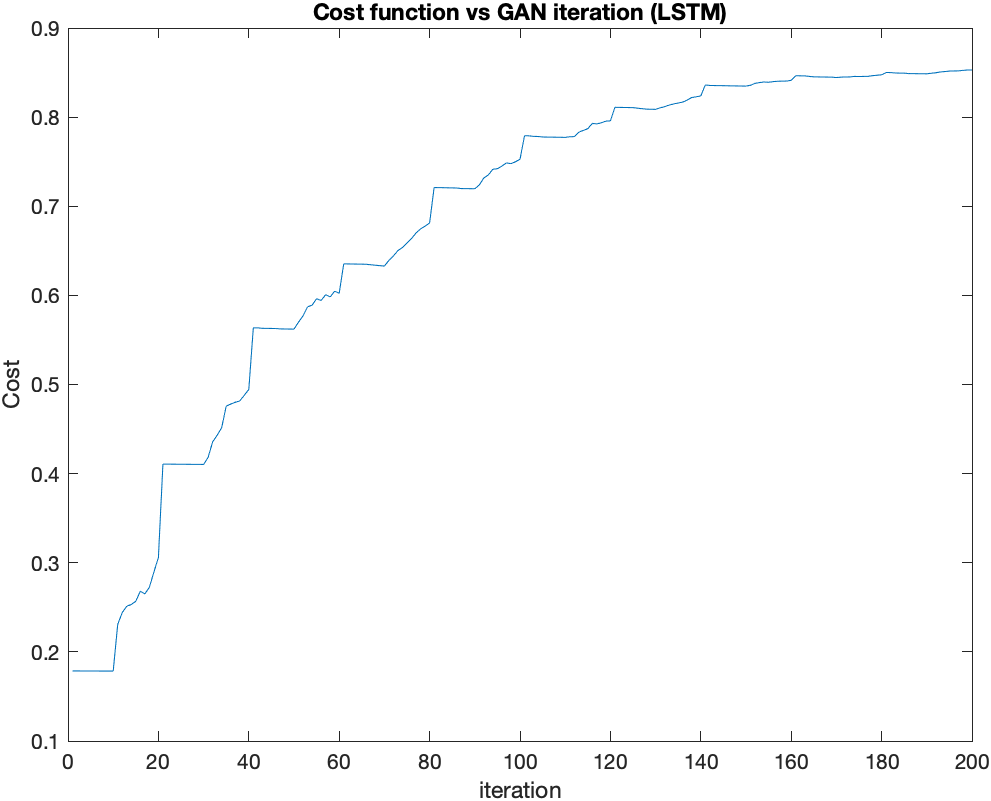
\includegraphics[angle=0,scale=.6]{testcost}
    \caption{Cost function on test data}
\end{figure}

\begin{figure}[h]
    \centering
    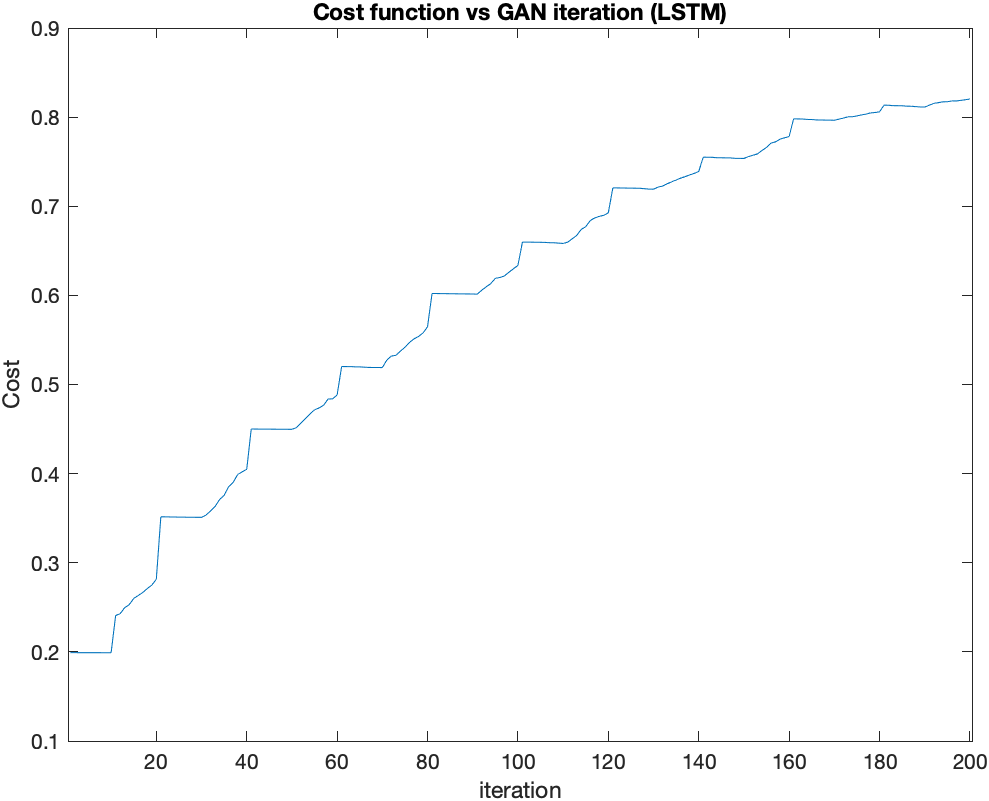
\includegraphics[angle=0,scale=.6]{costfunction}
    \caption{Cost function on AR(1) generated data}
\end{figure}

\begin{figure}[h]
    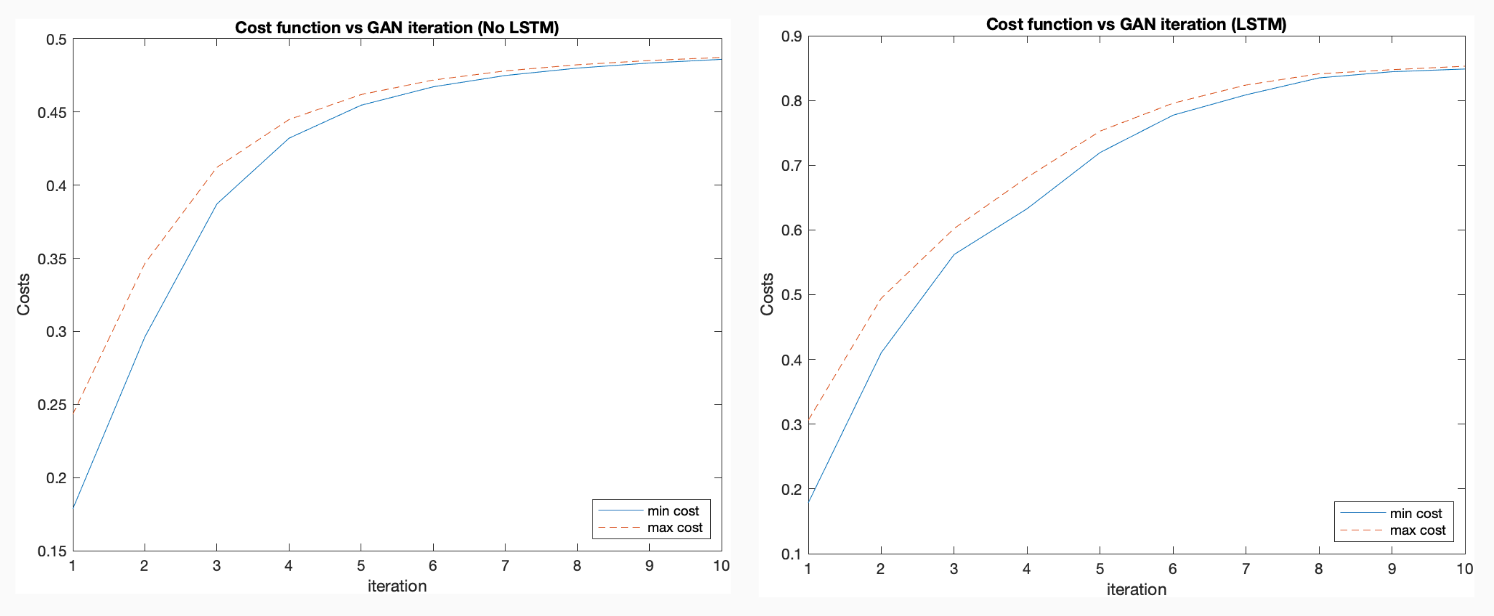
\includegraphics[angle=0,scale=.6]{testdata}
    \caption{Cost function on both GANs run on the given test data}
\end{figure}

\begin{figure}[h]
    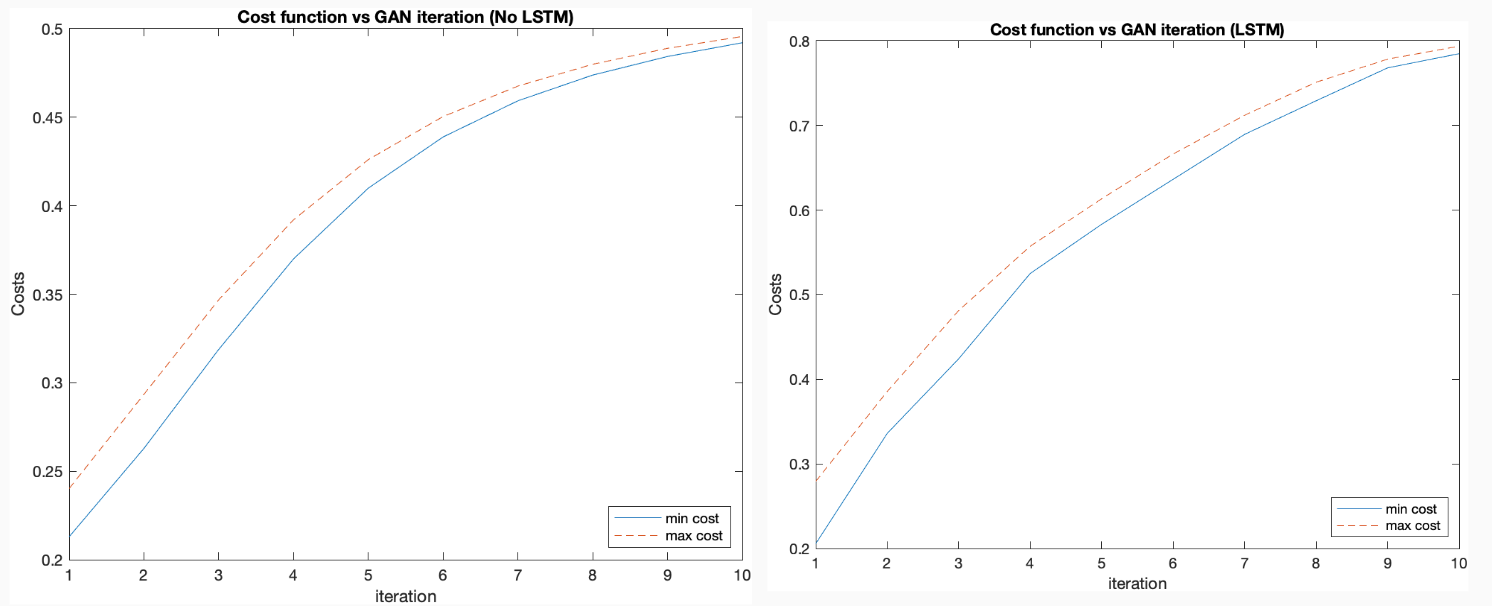
\includegraphics[angle=0,scale=.6]{randomdata}
    \caption{Cost function on both GANs run on random (normally distributed) data}
\end{figure}

\begin{figure}[h]
    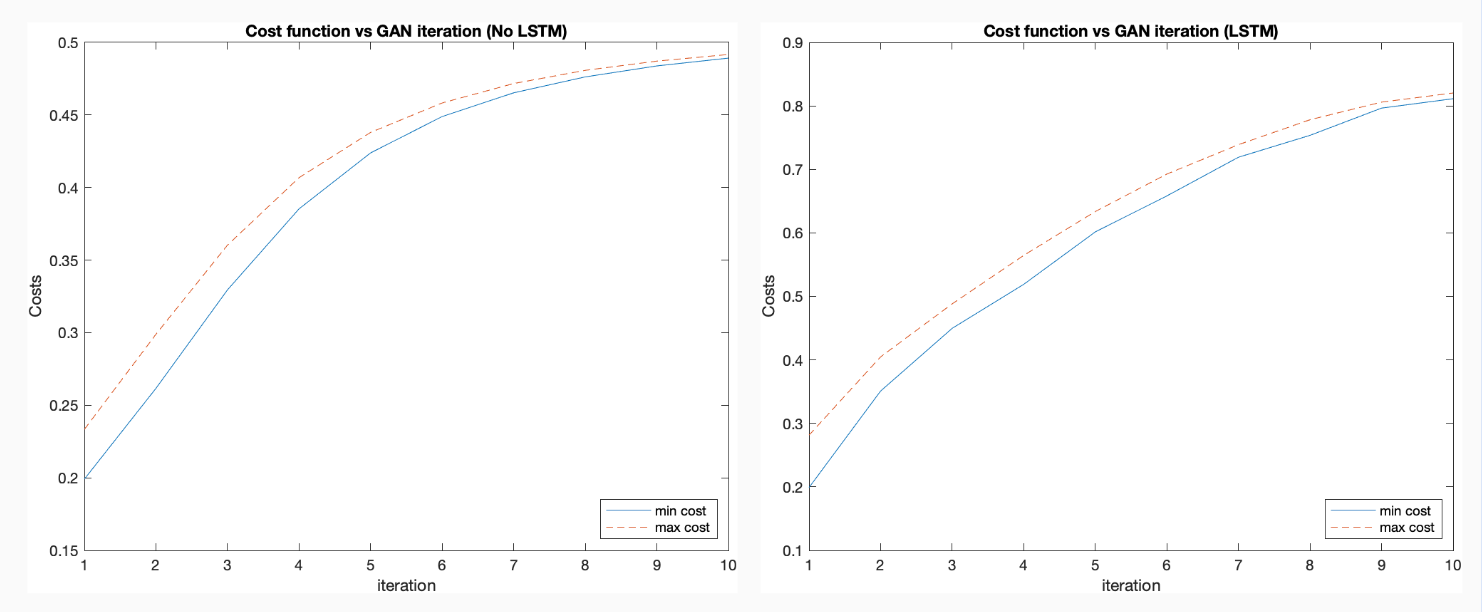
\includegraphics[angle=0,scale=.6]{generateddata}
    \caption{Cost function on both GANs run on data generated by the AR(1) model}
\end{figure}
\ \\
\ \\
\ \\
\ \\
\section{Conclusions}
We think there are some problems with this model. We will first note that there is always the possibility of an error in our code. One big concern of ours was that the minimzation phase seemed to be very ineffectual. This was particularly a concern in our project because we only implemented the LSTM in the minimzation phase. We tried implementing many different SG iterations per phase and still found that there was very little minimization occuring. We think that implementing a changing learning rate might make the process work better. We would recommend that future students re-examine this code and determine why the minimzation phase appears to have such a small impact. 

Another big problem was that cost function jumped a lot after the first stochastic gradient (SG) iteration for every maximization phase. We would expect the cost function to relatively zigzag between maximization and minimization phases, but this was not quite the case. We think this is a most likely area to have a bug in the code, but it is also possible that the gradient with respect to \(\mathbf{g}\) is extremely sensitive to changes in \(\omega\). Here we would again recommend tinkering with the learning rate in order to stabilize the change in the cost function. It is also possible that the maximization phase had such different behavior because it was not integrated with the LSTM. A good area for future exploration would be to integrate the LSTM with the entire GAN architecture.

These two problems were likely the biggest reason why we did not see much difference between the GAN + LSTM and the regular GAN. Because the LSTM was integrated in the minimzation phase, we believe that fixing the lack of minimzation would lead to much better results.

\end{document}
